\chapter{Rešerše}
\label{1-reserse}

\section{Volba metody pro tvorbu webové aplikace}

Při volbě, jakou metodu pro tvorbu aplikace použít, se nabízelo několik
%% ML: napr. za pouziti
%% ML: Vas vicet neni rozhodne konecny
možností jak ji vytvořit. Aplikace by mohla být vytvořena za použití
skriptovací jazyka PHP, Javascriptu nebo například Python frameworku 
pro tvorbu webových aplikací. 

Ze zadání projektového týmu ovšem vyplynulo, že by aplikace měla být
napsána v jazyce Python, a to z důvodu udržitelnosti kódu. Volba tedy
padla na Python frameworky.

\section{Volba Python frameworku}
Frameworkem je označována platforma, která se používá pro tvorbu aplikací. 
Je to soubor podpůrných programů a knihoven, které mají za cíl usnadnit 
jejich vývoj. Výběr vhodného frameworku byl vzhledem k jejich množství 
složitý. Mezi hlavní kritéria pro výběr frameworku se proto zařadila snadná
%% ML:: pokud trvate na anglictine, tak alespon do uvozovek
práce s databází, implementace per object permissions a dostupnost 
výukových materiálů a komunitní podpora. Díky těmto kritériím se nakonec 
vybíralo ze dvou frameworků, a to Flask a Django.

\begin{figure}[H] \centering
    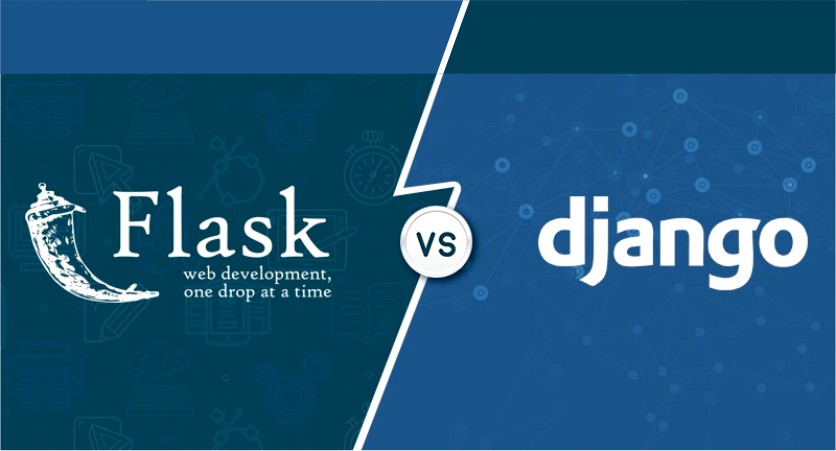
\includegraphics[width=240pt]{./pictures/1-django-vs-flask.jpeg}
    \caption[Flask vs Django]{Flask vs Django \cite{django-vs-flask}}
	\label{fig:Flask vs Django}                                
\end{figure}

Flask je open source webový framework napsaný v Pythonu, klasifikovaný
jako mikro z důvodu, že není potřeba žádných dodatečných knihoven ani
jiných nástrojů. Do Flasku lze ovšem doinstalovat různá rozšíření,
která v základní verzi chybí jako například Flask-Admin, což je
administrátorské rozhraní pro správu uživatelů a objektů v
databázi. Výhodou je jeho velká obliba v komunitě, kdy v roce 2020 měl
druhé místo na GitHubu z webových frameworků, a díky tomu disponuje
spoustou materiálů a tutoriálů. Avšak velká nevýhoda Flasku pro vývoj
naší aplikace je, že nedisponuje datovými modely. Pokud bychom v průběhu
vývoje chtěli přidat sloupec do naší databáze, musíme to udělat ručně
v databázi a poté ho přidat do třídy ve webové aplikaci. \cite{flask}

Django je nejpoužívanějším open source frameworkem. Jednou z jeho funkcí je že
disponuje objektově relačním mapováním. Jeho vlastností je tedy možnost generovat
model z databáze, který se zde může upravovat a poté jednoduchými
příkazy promítnout úpravy zpět do databáze. Další výhodou je implementované
administrátorské rozhraní a možnost doinstalováním přídavných balíčků,
poskytující jak grafické úpravy, tak přidané funkce. Jedním z nich je
i balíček django-guardian zajišťující podporu per object permissions. \cite{django}


Z těchto frameworků byl nakonec vybrán pro tvorbu aplikace framework
Django. Ten oproti Flasku disponoval snadnou a rychlou práci s modelem
databáze. Další výhodou je vývojáři implementované administrátorské
rozhraní, které se nemusí doinstalovat pomocí přídavného balíčku. Z
hlediska popularity a dostupnosti výuko\-vých materiálu jsou na tom oba
frameworky podobně, kdy se oba řadí na první dvě místa výrazně před
ostatní frameworky.

\vspace{10px}

\section{Volba databáze}

Jedním z hlavních úkolů bylo vytvoření databáze, ze které se budou
zobrazovat poskytnutá data z projektu Viskalia, rozšířená o další
položky. Textová data zpro\-středkovaná Národním muzem byla uložena v
MariaDB databázi a obrazová data byla v souborovém systému. Příslušná
databáze ovšem postrádá jakoukoli normalizaci a data obsahují spoustu
duplicit. Nabízí se proto otázka, zda provést normalizaci dat a opět
použít relační databázi, nebo použít nějakou z nerelačních
%% ML: vetu prepiste, opakovani slova "problem"
databází. Asi zásadní problém s NoSQL databází, který by mohl nastat
je problém v komunikaci s frameworkem pro vývoj webových aplikací. Ty
v zásadě nemají problém komunikovat s jakýmkoliv typem relační
databáze, ovšem často nemají engine pro databáze typu NoSQL. Zvolili
jsme tedy relační databázi, a to MariaDB z důvodu poskytnutí dat právě
z tohoto databázového systému. \cite{django} \cite{mariadb}

\newpage

\section{Automatizace nasazení aplikace}

%% ML: deployment v zavorce anebo alespon v uvozovkach
Jedním z hlavních úkolů je také automatizace deploymentu aplikace a
zajištění bezproblémového chodu na všech zařízeních. Při této otázce
jsme se nejprve museli rozhodnout, na jakém operačním systému se bude
aplikace vyvíjet a následně bude provozována. Po kratší úvaze jsme
zvolili systém Linux, který je vhodnější zejména pro vývoj aplikací v
jazyce Python. Zde jsme tedy hledali vhodný software pro
kontejnerizaci naší vyvíjené aplikace. Hlavními důvody pro jejich
použití je, že obsahují kompletní prostředí pro vývoj a chod aplikace
jako jsou knihovny nebo konfigurační soubory. Aplikace a všechny její
komponenty většinou běží v několika kontejnerech, které spolu dokáží
komunikovat. Jejich chod je od zbytku systému oddělen. Zde se nabízejí
dvě varianty, a to jsou LXC (LinuX Containers) anebo Docker, což jsou
jedny z nejpoužívanějších aplikací. Hlavní rozdíl mezi těmito
aplikacemi je, že kontejnery LXC obsahují svůj vlastní operační systém
a působí tedy spíše jako virtuální počítač. Docker oproti tomu žádné
takové prostředí nemá a běží pouze separovaně na operačním systému
uživatele. Dalším hlavním rozdílem je větší propracovanost Dockeru,
které umožňuje více nastavení kontejnerů a rozdělení aplikace do více
kontejnerů. Oproti LXC může být Docker použit i na
jiném operačním systému než je Linux. Z těchto důvodů byl pro
kontejnerizaci zvolen Docker. \cite{deployment}

\newpage

\section{Normalizace databáze}

Normalizace databáze je reorganizace dat podle normalizačních standardů. 
Používá se pro snížení nadbytečných dat v databázi, například při duplicitách 
ve sloupcích. Normalizačních forem je pět, ale zpravidla se používají pouze 
první tři stupně. Jednotlivé stupně na sebe navzájem navazují, pokud budeme 
tedy chtít uplatnit třetí normalizační stupeň, musíme nejprve provést první a druhý.

První stupeň je v zásadě použití selského rozumu. Jedná se o odstranění 
duplicitních sloupců a sloupců, jež jsou kombinací jiných sloupců.

Druhý stupeň nám říká, že duplicitní hodnoty by měly být z tabulky odstraněny 
a přesunuty do nové tabulky, která je propojená cizím klíčem. Z tabulky se tedy 
odstraní všechny hodnoty, které platí pro více záznamů.

Třetí stupeň udává, že by tabulka neměla obsahovat hodnoty, které jsou na sobě závislé. 

Ve čtvrtém stupni by záznamy neměly obsahovat více nezávislých hodnot jedné podmnožiny. 
Takovéto hodnoty by opět mely být převedeny do samostatné tabulky a spojeny cizím klíčem.

Pátý stupeň platí, pokud není možné tabulku dále dělit bez ztráty dat. Po 
rozdělení by došlo ke ztrátě vztahů, které mezi daty platí. \cite{normalizace}






















